\documentclass[]{article}
\usepackage[T1]{fontenc}
\usepackage[utf8]{inputenc}
%\usepackage[icelandic]{babel}
\usepackage{caption}
\usepackage{circuitikz}
\usepackage{grffile} 
\usepackage[margin=1in]{geometry}

% grffile er pakki sem leifir manni að nota "" til þess að forðast að nota
% nafnið á myndinni með.
\usepackage{graphicx}
% \graphicspath{{images/}} Sýnir undir möppu þar sem myndirnar eru

\usepackage{hyperref}
%fyrirlinka - \url{www.....}
\begin{document}


\title{Formleg mál og reiknanleiki}
\author{Pétur}
\maketitle

\section*{1.}

\subsection*{a)}
$A = \{0^{n+m}1^{m}| n \geq 0, m \geq 0 \}$ \\
\begin{itemize}
	\item Assume A is regular only if pumping lemma holds for some p.
	\item Let $s = 0^{p}1^{p}$, so that $|s| = 2p > p$.
	 According to pumping lemma, s can be split into 3 pieces, 				$s=xyz$, such that $xy^{i}z \epsilon A$ for all $i \geq 0$.
	\item 3 cases
	\begin{enumerate}
		\item y consist only of zeros: $xy^{2}z$ has more zeros than 		ones and that is not in the language A.
		\item y consist solely on ones: $xy^{2}z$  has more ones 				than zeros and that is not in the language A.
		\item y consist of "10": $xy^{2}z$ has then "1010" which is 			not in the language A.
	\end{enumerate}
	\item as all three cases lead to contradiction, the initial assumption, A being regular must be false.
\end{itemize}

\subsection*{b)}
$B = \{0^{n}1^{m}0^{n}|n \geq 0, m \geq 0\}$

\begin{itemize}
	\item Assume B is regular only if pumping lemma holds for some p.
	\item Let $s = 0^{p}10^{p}$, so that $|s| = 2p > p$. According to pumping lemma, s can be split into 3 pieces, $s = xyz$, such that $xy^{i}z \epsilon B$ for all $i\ge0$.
	\item 3 cases
	\begin{enumerate}
		\item y consist only of zeros left hand side of the one: 				$xy^{2}z$ has more zeros left hand side than right, which is 		not in the language B.
		\item y consist only of zeros right hand side of the one: 				$xy^{2}z$ has more zeros right hand side than left, which is 		not in the language B.
		\item y consist of "010": $xy^{2}z$ the string contains then 		"010010" which is not in the language B.
	\end{enumerate}
	\item as all three cases lead to contradiction, the initial assumption, B being regular must be false.
\end{itemize}

\pagebreak

\subsection*{c)}
$C = \{www|w\epsilon \{0,1\}*\}$
\begin{itemize}
	\item Assume C is regular only if pumping lemma holds for some p.
	\item Let $s = 0^{p}10^{p}10^{p}1$, so that $|s| = 3p > p$. According to pumping lemma, s can be split into 3 pieces, $s = xyz$, such that $xy^{i}z \epsilon C$ for all $i\ge0$.
	\item 3 cases
	\begin{enumerate}
		\item y consist only of zeros left hand side: 				$xy^{2}z$ has more zeros left hand side than right and middle, which is 		not in the language C.
		\item y consist only of zeros right hand side : 				$xy^{2}z$ has more zeros right hand side than left and middle, which is 		not in the language C.
		\item y consist of zero in the middle: $xy^{2}z$ the string contains then more zeros in the middle than right and left hand site, which means that it is not in the language C.
	\end{enumerate}
	\item as all three cases lead to contradiction, the initial assumption, C being regular must be false.
\end{itemize}

\section*{2.}

$A = \{x = y + z | x,y,z$ are binary integers and x is the sum of y and z $\}$ \\
\begin{itemize}
	\item Assume A is regular only if pumping lemma holds for some p	
	\item x,y,z are not pump able. If they are chosen as $y^{2}$ that means it will change the outcome of the calculation.
	\item as all three cases lead to contradiction, the initial assumption, A being regular must be false.
\end{itemize}
\section*{3.}

\subsection*{a)}

Let $F = \{a^{i}b^{j}c^{k} | i,j,k \ge 0$, and if $i = 1$ then $j = k\}$

\begin{itemize}
	\item Assume F is regular only if pumping lemma holds for some p
	\item let $s = a^{p}b^{p}c^{p}$, so that $|s| = 3p > p$. According to pumping lemma s = xyz, such that $xy^{i}z$ $\epsilon$ C for all $i \ge 0$.
	\item 3 cases
	\begin{enumerate}
		\item y consist of "ab": $xy^{2}z$ which generates "abab" which is not in the language F.
		\item y consist of "abc": $xy^{2}z$ which generates "abcabc" which is not in the language F.
		\item y consist of "bc": $xy^{2}z$ which generates "bcbc" which is not in the language F.
	\end{enumerate}
	\item as all three cases lead to contradiction, the initial assumption, A being regular must be false.
\end{itemize}

\pagebreak

\subsection*{b)}
\begin{itemize}
\item 3 cases
	\begin{enumerate}
		\item y consist of "a": $xy^{2}z$ which generates "aa" which is in the language F.
		\item y consist of "b": $xy^{2}z$ which generates "bb" which is in the language F.
		\item y consist of "c": $xy^{2}z$ which generates "cc" which is in the language F.
	\end{enumerate}
	\item as all three cases lead to no contradiction, the initial assumption, F being regular must be true.
\end{itemize}

\subsection*{c)}
They do not contradict the pumping lemma because the pumping lemma says that if you can pump any y and it is in the language then the language must be regular. So it depends on what y you chose. One can show irregularity and other can show regularity but both are able to pump. While you are proving that language is not regular than you chose the y that you are pumping to show the irregularity.

\section*{4.}

\subsection*{a)}
The NFA that will recognize will start with
\begin{itemize}
	\item k number of a "a" or "b" for each k.
	\item when k-1 has bin reach then it ends with a.
	\item That means that you need infinite amount of states to manage all the "a" transition. So that the state machine knows when it should quit and end with k-1 "a".
\end{itemize}

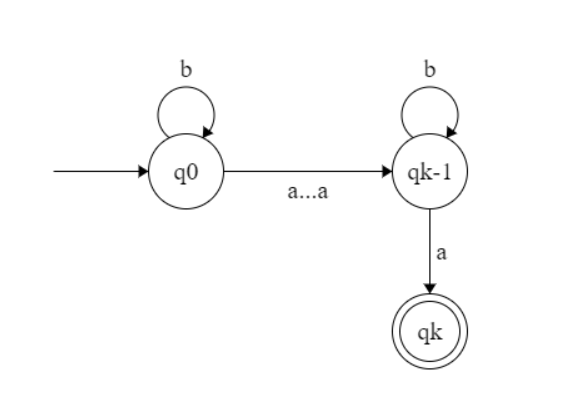
\includegraphics[scale=1]{mynd}
\subsection*{b)}

\end{document}